\documentclass{report}
\usepackage{amsmath}
\usepackage{amssymb}
\usepackage{graphicx}
\usepackage{tcolorbox}

\newtcolorbox{mybox}{colback=red!5!white,colframe=red!75!black}

\title{Winter 2022 MTH 261 Mini Test 1}
\author{Marvin Lin}
\date{January 2022}

\begin{document}

\maketitle

\section*{Question 1}

\begin{mybox}
Consider the system of equations bellow:
\begin{alignat*}{4}
 x & {}-{} & 7y & {} {} &    {}+{} & 6t & {}={} &  5 \\
   & {} {} &    & {} {} &  z {}-{} & 2t & {}={} & -3 \\
-x & {}+{} & 7y & {}-{} & 4z {}+{} & 2t & {}={} &  7
\end{alignat*}
(a) Write the system of equations as a vector equation.\\
(b) Write the system as a matrix equation A\textbf{x}=\textbf{b}\\
(c) Solve the system of equations using linear algebra techniques. Indicate your solution in parametric vector form.
\end{mybox}

\subsubsection*{Part (a)}
\begin{equation}
\begin{bmatrix} x \\ 0 \\ -x \end{bmatrix}
+
\begin{bmatrix} -7y \\ 0 \\ 7y \end{bmatrix}
+
\begin{bmatrix} 0 \\ z \\ -4z \end{bmatrix}
+
\begin{bmatrix} 6t \\ -2t \\ 2t \end{bmatrix}
=
\begin{bmatrix} 5 \\ -3 \\ 7 \end{bmatrix}
\end{equation}

\begin{equation}
x
\begin{bmatrix} 1 \\ 0 \\ -1 \end{bmatrix}
+
y
\begin{bmatrix} -7 \\ 0 \\ 7 \end{bmatrix}
+
z
\begin{bmatrix} 0 \\ 1 \\ -4 \end{bmatrix}
+
t
\begin{bmatrix} 6 \\ -2 \\ 2 \end{bmatrix}
=
\begin{bmatrix} 5 \\ -3 \\ 7 \end{bmatrix}
\end{equation}

\subsubsection*{Part (b)}
\begin{equation}
\begin{bmatrix}
1 & -7 & 0 & 6 \\ 
0 & 0 & 1 & -2 \\ 
-1 & 7 & -4 & 2 
\end{bmatrix}
\begin{bmatrix}
x \\ 
y \\ 
z \\
t
\end{bmatrix}
=
\begin{bmatrix} 
5 \\ 
-3 \\ 
7
\end{bmatrix}
\end{equation}

\subsubsection*{Part (c)}
\begin{equation}
\begin{bmatrix}
1 & -7 & 0 & 6 & 5 \\ 
0 & 0 & 1 & -2 & -3 \\ 
-1 & 7 & -4 & 2 & 7
\end{bmatrix}
\end{equation}
\begin{equation}
\sim
\begin{bmatrix}
1 & -7 & 0 & 6 & 5 \\ 
0 & 0 & 1 & -2 & -3 \\ 
0 & 0 & -4 & 8 & 12
\end{bmatrix}
\end{equation}
\begin{equation}
\sim
\begin{bmatrix}
1 & -7 & 0 & 6 & 5 \\ 
0 & 0 & 1 & -2 & -3 \\ 
0 & 0 & 0 & 0 & 0
\end{bmatrix}
\rightarrow
RREF
\end{equation}
\begin{equation*}
\therefore
x-7y+6t=5
\rightarrow
x=5+7y-6t
\end{equation*}
\begin{equation*}
y=y
\end{equation*}
\begin{equation*}
z-2t=-3
\rightarrow
z=-3+2t
\end{equation*}
\begin{equation*}
t=t
\end{equation*}
\begin{equation}
\mathbf{x}
=
\begin{bmatrix}
x \\ 
y \\ 
z \\
t
\end{bmatrix}
=
\begin{bmatrix}
5+7y-6t \\ 
y \\ 
-3+2t \\
t
\end{bmatrix}
=
\begin{bmatrix}
5 \\ 
0 \\ 
-3 \\
0
\end{bmatrix}
+
\begin{bmatrix}
7y \\ 
y \\ 
0 \\
0
\end{bmatrix}
+
\begin{bmatrix}
6t \\ 
0 \\ 
2t \\
t
\end{bmatrix}
=
\begin{bmatrix}
5 \\ 
0 \\ 
-3 \\
0
\end{bmatrix}
+
y
\begin{bmatrix}
7 \\ 
1 \\ 
0 \\
0
\end{bmatrix}
+
t
\begin{bmatrix}
6 \\ 
0 \\ 
2 \\
1
\end{bmatrix}
\end{equation}

\clearpage
\section*{Question 2}

\begin{mybox}
\begin{equation*}
Let \: \mathbf{u}=\begin{bmatrix} 1 \\ -2 \\ 2 \\ \end{bmatrix},\mathbf{v}=\begin{bmatrix} 0 \\ 5 \\ 5 \\ \end{bmatrix},\mathbf{w}=\begin{bmatrix} -2 \\ 0 \\ -8 \\ \end{bmatrix},\mathbf{b}=\begin{bmatrix} -1 \\ -11 \\ -6 \\ \end{bmatrix}.
\end{equation*}
\begin{equation*}
Is \: \mathbf{b}\in\mathrm{span}\{\mathbf{u}, \mathbf{v}, \mathbf{w}\}?
\end{equation*}
\end{mybox}

\begin{equation}
\begin{bmatrix}
1 & 0 & -2 \\ 
-2 & 5 & 0 \\ 
2 & 5 & -8 \\ 
\end{bmatrix}
\end{equation}
\begin{equation}
\sim
\begin{bmatrix}
1 & 0 & -2 \\ 
-2 & 5 & 0 \\ 
0 & 10 & -8 \\ 
\end{bmatrix}
\end{equation}
\begin{equation}
\sim
\begin{bmatrix}
1 & 0 & -2 \\ 
0 & 5 & -4 \\ 
0 & 10 & -8 \\ 
\end{bmatrix}
\end{equation}
\begin{equation}
\sim
\begin{bmatrix}
1 & 0 & -2 \\ 
0 & 5 & -4 \\ 
0 & 0 & 0 \\ 
\end{bmatrix}
\rightarrow
REF
\end{equation}
\begin{equation}
\sim
\begin{bmatrix}
1 & 0 & -2 \\ 
0 & 1 & -4/5 \\ 
0 & 0 & 0 \\ 
\end{bmatrix}
\rightarrow
RREF
\end{equation}
\begin{equation*}
\mathbf{u}
=-2;
\mathbf{v}
=-4/5;
\mathbf{w}
=
\mathbf{w}
\end{equation*}
\begin{equation}
\textbf{b}
=
\begin{bmatrix}
-1 \\ 
-11 \\ 
-6 \\ 
\end{bmatrix}
\neq
\begin{bmatrix}
-2 \\ 
-4/5 \\ 
\mathbf{w} \\ 
\end{bmatrix}
\end{equation}
Since the equation above is a false statement, the following can be determined:
\begin{equation}
\therefore
\textbf{b}
\notin
\mathrm{span}\{\mathbf{u}, \mathbf{v}, \mathbf{w}\}
\end{equation}

\clearpage
\section*{Question 3}

\begin{mybox}
\begin{equation*}
Let \: \mathbf{u}=\begin{bmatrix} -3 \\ 2 \\ \end{bmatrix} \: and \: \mathbf{v}=\begin{bmatrix} -1 \\ -6 \\  \end{bmatrix}.
\end{equation*}
\begin{center}
Draw a Cartesian plane to draw the following graphs on.\\ Graph \textbf{u}, \textbf{v}, 2\textbf{u}, -\textbf{v}, 2\textbf{u} - \textbf{v}.
\end{center}
\end{mybox}

\begin{equation*}
\textbf{u}
=
\begin{bmatrix}
-3 \\
2
\end{bmatrix}
;
\textbf{v}
=
\begin{bmatrix}
-1 \\
-6
\end{bmatrix}
;
2
\textbf{u}
=
2
\begin{bmatrix}
-3 \\
2
\end{bmatrix}
=
\begin{bmatrix}
-6 \\
4
\end{bmatrix}
;
-
\textbf{v}
=
-1
\begin{bmatrix}
-1 \\
-6
\end{bmatrix}
=
\begin{bmatrix}
1 \\
6
\end{bmatrix}
\end{equation*}
\begin{equation*}
2
\textbf{u}
-
\textbf{v}
=
2
\begin{bmatrix}
-3 \\
2
\end{bmatrix}
-
\begin{bmatrix}
-1 \\
-6
\end{bmatrix}
=
\begin{bmatrix}
-6 \\
4
\end{bmatrix}
-
\begin{bmatrix}
-1 \\
-6
\end{bmatrix}
=
\begin{bmatrix}
-5 \\
10
\end{bmatrix}
\end{equation*}
\begin{figure}[h]
  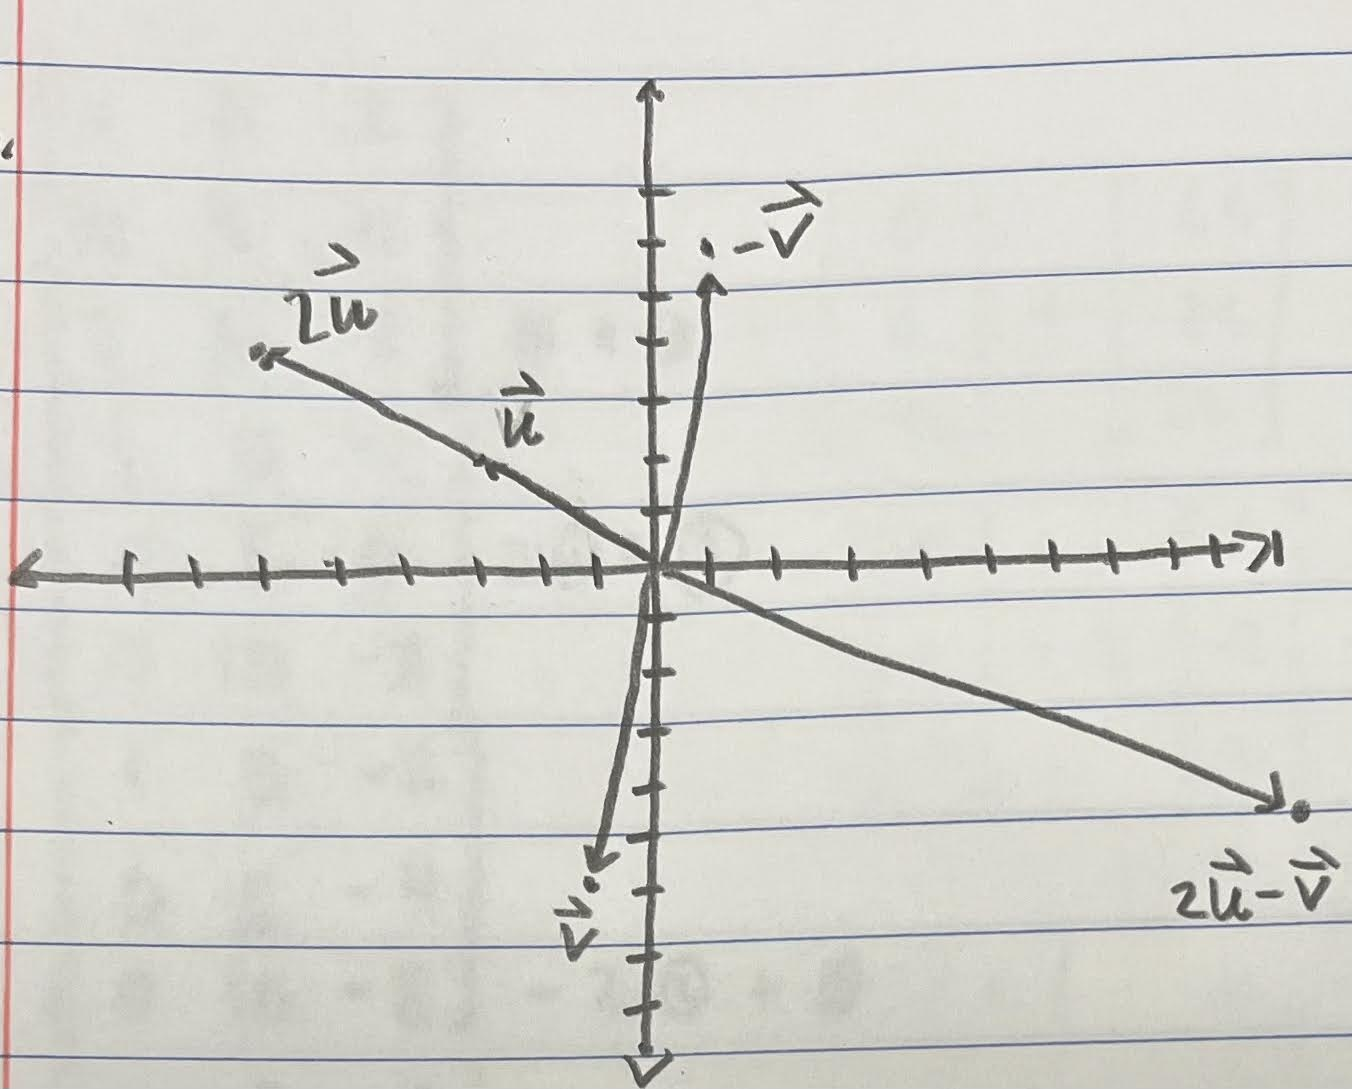
\includegraphics[width=\linewidth]{graph.jpg}
  \caption{Graph of vectors}
  \label{fig:graph1}
\end{figure}
\end{document}
